\documentclass{beamer}

% \usepackage{taltech_bsc}
\usepackage[estonian]{babel}
\usepackage{graphicx}
\graphicspath{{../figures/}}
\usepackage{bm}

% \usefonttheme{serif}
% Remove navigation bar
% \setbeamertemplate{navigation symbols}{}
% \usetheme{Singapore}
\usetheme{seville}
% \setbeamertemplate{footline}[frame number]

\newcommand{\del}{\ensuremath{\partial}}
\DeclareMathOperator{\D}{d}
\DeclareMathOperator{\sech}{sech}
\newcommand{\ft}{\mathcal{F}}
\newcommand{\ift}{\mathcal{F}^{-1}}

\title{Graph Neural Networks}
% \subtitle{bakalaureusetöö}
\author{Mikk Kruusalu}
\date{}

\begin{document}

\begin{frame}
    \titlepage
\end{frame}

\begin{frame}{Graphs}
    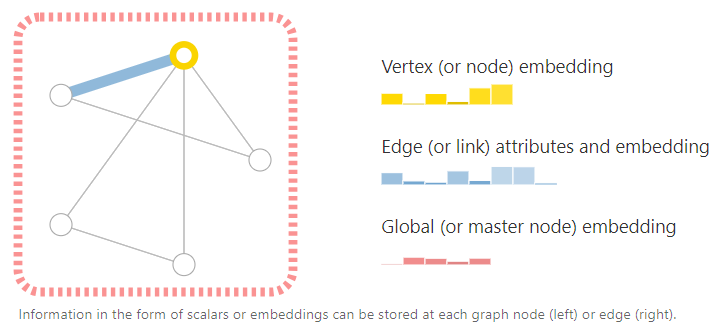
\includegraphics[width=\textwidth]{image.png}
    \let\thefootnote\relax\footnote{\url{distill.pub/2021/gnn-intro}}

    \vspace{-0.7cm}
    \begin{itemize}
        \item $G = (\mathcal{V}, \mathcal{E})$
        \item features
    \end{itemize}

\end{frame}

\begin{frame}{Graphs}
    \begin{itemize}
        \item images,
        \item molecules,
        \item social interactions,
        \item route planning and logistics,
        \item disease spread
    \end{itemize}
\end{frame}

\begin{frame}{Adjacency matrix}
    Each node $u\in\mathcal{V}$ has features $\mathbf{h}_u\in\mathbb{R}^{m}$ \\
    Each edge $(u,v)\in\mathcal{E}$ has features $\mathbf{h}_{(u,v)}\in\mathbb{R}^{k}$
    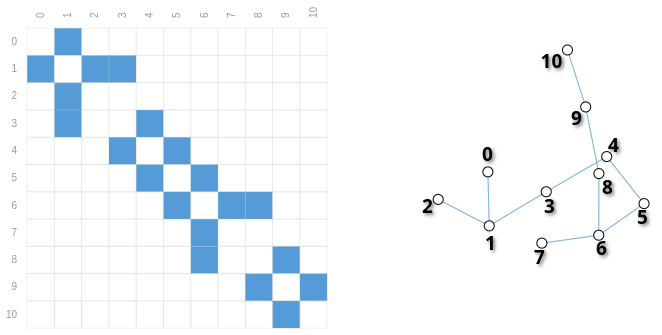
\includegraphics[width=\textwidth]{adjacency.png}
    \let\thefootnote\relax\footnote{\url{distill.pub/2021/gnn-intro}}

    \vspace{-0.7cm}
    \begin{itemize}
        \item directed edges,
        \item weighted edges
    \end{itemize}
\end{frame}

\begin{frame}{Tasks}
    \begin{itemize}
        \item Graph-level
        \item Node-level
        \item Edge-level
    \end{itemize}

    The task is ultimately defined by the loss function.
\end{frame}

\begin{frame}{Message passing}
    \begin{align*}
        &\textsf{nodes}& \mathbf{m}_u^k &= \textsc{aggregate}(\{\mathbf{h}_v^k,\ \forall v\in\mathcal{N}(u)\}) \\
        & & \mathbf{h}_u^{k+1} &= \textsc{update}(\mathbf{h}_u^k, \mathbf{m}_u^k) \\
        &\textsf{edges}& \mathbf{h}_{(u,v)}^{k+1} &= \textsc{update}(\mathbf{h}_{(u,v)}^k, \mathbf{h}_u^k, \mathbf{h}_v^k)
    \end{align*}
    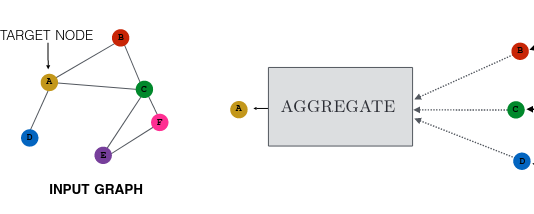
\includegraphics[width=\textwidth]{message_passing.png}
    \let\thefootnote\relax\footnote{W. L. Hamilton, \textit{Graph Represantation Learning}, Synthesis Lectures on Artificial Intelligence and Machine Learning, vol. 14, no. 3, 2020}
\end{frame}

\begin{frame}{Example}
    Simplest approach
    \begin{align*}
        &\textsf{message}& \mathbf{m}_u^k &= \sum_{v\in\mathcal{N}(u)} \frac{\mathbf{h}_v^k}{\sqrt{ |\mathcal{N}(u)| |\mathcal{N}(v)| }} \\
        &\textsf{update}& \mathbf{h}_u^{k+1} &= \sigma \left( \mathbf{W}_{self} \mathbf{h}_u + \mathbf{W}_{neigh}\mathbf{m}_u^k + \mathbf{b}_u \right)
    \end{align*}

\end{frame}

\begin{frame}{Attention}
    Define attention weights
    \begin{equation*}
        \alpha_{u, v} = \frac{\exp(\mathbf{a}^\intercal \cdot \mathbf{W}[\mathbf{h}_u, \mathbf{h}_v])}
        {\sum_{v'\in\mathcal{N}(u)} \exp(\mathbf{a}^\intercal \cdot \mathbf{W}[\mathbf{h}_u, \mathbf{h}_{v'}])}
    \end{equation*}
    $[\mathbf{h}_u, \mathbf{h}_{v'}]$ means a concatenation of the hidden vectors, $\mathbf{a}$ is the attention vector that is trainable parameter with the weight matrix $\mathbf{W}$.

    Message is then weighted by attention
    \begin{equation*}
        \mathbf{m}_u = \sum_{v\in\mathcal{N}(u)} \alpha_{u,v}\mathbf{h}_v.
    \end{equation*}

\end{frame}

\begin{frame}{Skip connections}
    Add the previous state to the updated one
    \begin{equation*}
        \mathbf{h}_u^{k+1} = \bm{\alpha}\cdot \textsc{update}(\mathbf{h}_u^k, \mathbf{m}_u^k) + (1-\bm{\alpha}) \cdot \mathbf{h}_u^k
    \end{equation*}
    $\bm{\alpha} \in [0, 1]^m$ is a gating vector.
\end{frame}

\begin{frame}{Similarity to RNNs}
    Message passing is an iterative or recurrent process $\rightarrow$ possible to use RNN blocks for \textsc{update} function
    \begin{itemize}
        \item GRU -- hidden state is the previous $\mathbf{h}_u^{k-1}$ and the new data point is the message $\mathbf{m}_u^{k-1}$.
        \item LSTM -- define another feature vector per each node for cell state.
    \end{itemize}
\end{frame}

\begin{frame}{Applications}
    By the end of message passing we have the same graph with updated features.

    \begin{itemize}
        \item Node or edge level
        \begin{enumerate}
            \item define the node embeddings $\mathbf{z}_u = \mathbf{h}_u^K$,
            \item use regular loss functions, such as MSE or Cross-Entropy and sum the result over nodes.
        \end{enumerate}
        \item Graph-level
        \begin{enumerate}
            \item pool the updated graph to get $\mathbf{z}_G$. This can use any function -- maximum, average, MLP, etc,
            \item use regular loss functions and sum the result over graphs.
        \end{enumerate}
        \item Relation Prediction
        \begin{enumerate}
            \item predict the adjacency matrix,
            \item take the norm between predicted and real adjacency matrix.
        \end{enumerate}
    \end{itemize}
\end{frame}

\begin{frame}{Implementation}
    The library PyTorch Geometric (PyG)
    \begin{itemize}
        \item graph datasets,
        \item graph data batching,
        \item message passing,
        \item many convienience functions
    \end{itemize}
\end{frame}

\begin{frame}[plain]
    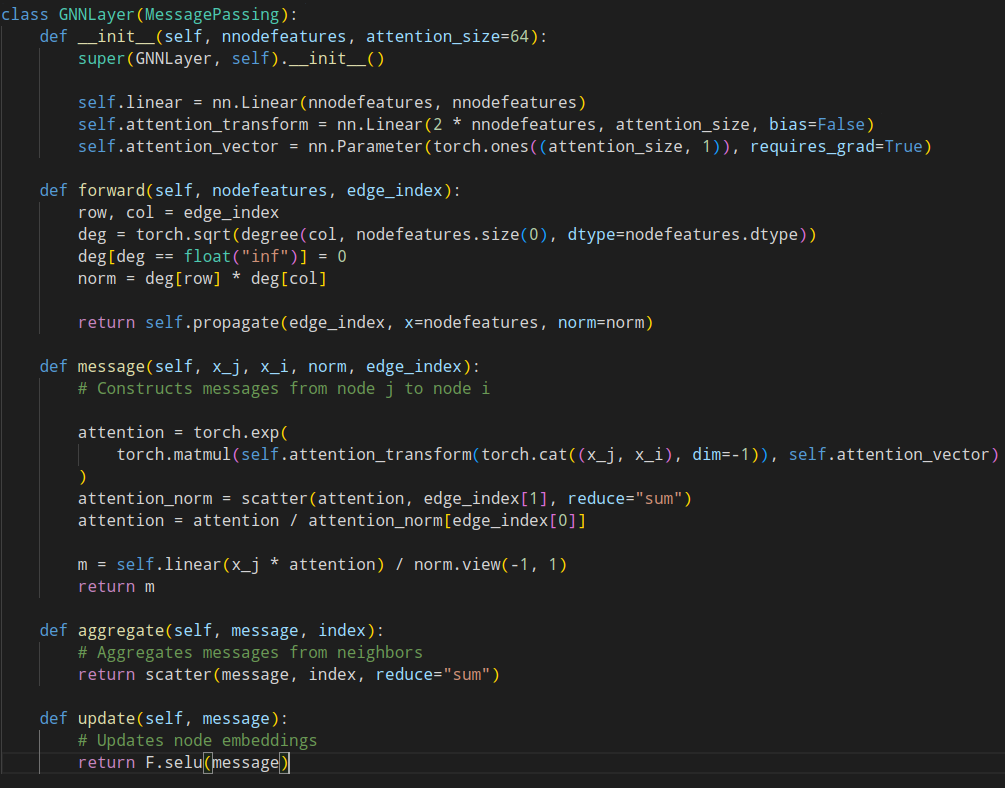
\includegraphics[width=\textwidth]{mp_code.png}
\end{frame}

\begin{frame}[plain]
    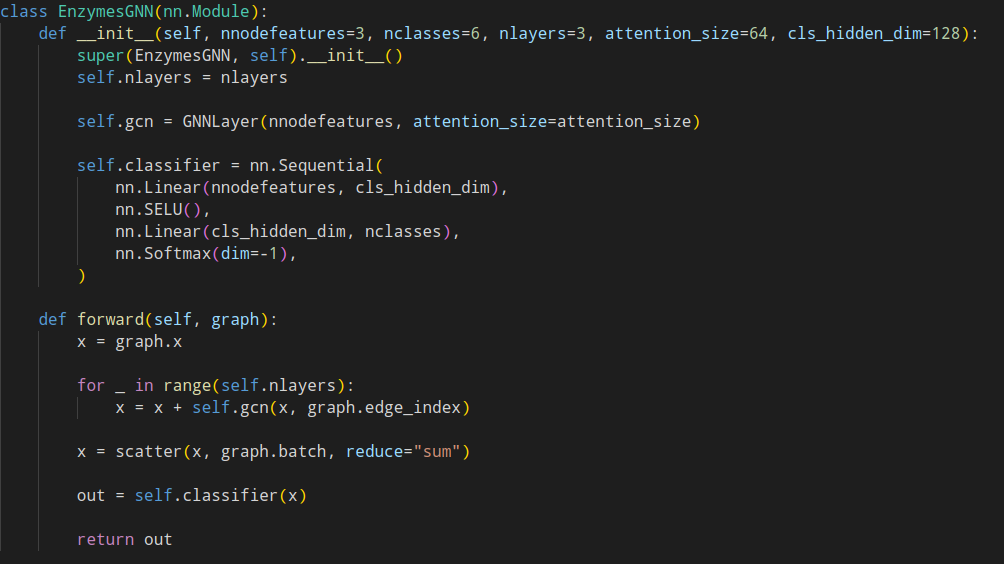
\includegraphics[width=\textwidth]{net_code.png}
\end{frame}

\begin{frame}
    W. L. Hamilton, \textit{Graph Represantation Learning}, Synthesis Lectures on Artificial Intelligence and Machine Learning, vol. 14, no. 3, 2020

    \url{distill.pub/2021/gnn-intro}

    \url{distill.pub/2021/understanding-gnns/}

    \vfill
    Code \url{github.com/mikk-kruusalu/deep_learning_project}
\end{frame}

\end{document}